% ==================== CHƯƠNG 7 ====================
\newpage
\chap{Hiện thực hệ thống}\label{sec:impl}

\sect{Kiến trúc tổng thể}\label{sec:arch}
Hệ thống theo kiến trúc nhiều tầng (Hình~\ref{fig:arch}): tầng nguồn dữ liệu, tầng ETL, tầng kho dữ liệu, tầng dịch vụ (OLAP API và mô hình DSS) và tầng trình bày (dashboard). Kho dữ liệu đóng vai trò \textbf{phân hệ quản lý dữ liệu} chung cho cả phân tích OLAP và DSS.

\begin{figure}[H]
\centering
\begin{tikzpicture}[node distance=0.5cm and 0.6cm,
  layer/.style={draw=gray!60, rounded corners=4pt, fill=gray!5, inner sep=6pt},
  box/.style={draw=heading1, fill=white, rounded corners=3pt, align=center, font=\footnotesize, text width=2.7cm, minimum height=1.0cm},
  arr/.style={-{Latex[length=2mm]}, thick, heading2}]
\node[box, fill=gray!12] (csv) {\textbf{CSV nguồn}\\ hour.csv, day.csv};
\node[box, right=of csv] (etl) {\textbf{ETL (Python)}\\ extract, transform,\\ load, validate};
\node[box, right=of etl, fill=heading1!10, text width=3.2cm] (dw) {\textbf{PostgreSQL}\\ schema \code{dw}: Star Schema\\ view \code{v\_rentals\_flat}};
\node[box, below=1.1cm of dw, text width=3.2cm] (api) {\textbf{FastAPI}\\ OLAP, KPI, climate\\ \code{/api/dss/*}};
\node[box, left=of api, fill=primary!12, draw=primary] (dss) {\textbf{Mô hình DSS}\\ \code{src/dss/engine.py}\\ ngưỡng, phân loại,\\ khuyến nghị};
\node[box, below=1.1cm of api, text width=3.2cm] (ui) {\textbf{Dashboard React}\\ Vite, Recharts\\ bộ lọc, KPI, OLAP, DSS};
\node[box, left=of ui, fill=gray!12] (user) {\textbf{Người dùng}\\ quản lý vận hành,\\ nhà phân tích};
\draw[arr] (csv) -- (etl); \draw[arr] (etl) -- (dw);
\draw[arr] (dw) -- node[right, font=\scriptsize] {SQL chỉ đọc} (api);
\draw[arr, <->] (api) -- (dss);
\draw[arr] (api) -- node[right, font=\scriptsize] {JSON / HTTP} (ui);
\draw[arr, <->] (ui) -- (user);
\end{tikzpicture}
\caption{Kiến trúc tổng thể hệ thống}
\label{fig:arch}
\end{figure}

\sect{Công nghệ sử dụng}
\begin{table}[H]
\centering
\caption{Công nghệ sử dụng}
\begin{tabularx}{\textwidth}{|p{3.2cm}|p{4.2cm}|X|}
\hline
\textbf{Tầng} & \textbf{Công nghệ} & \textbf{Lý do lựa chọn} \\ \hline
Kho dữ liệu & PostgreSQL~\cite{postgres} & Hỗ trợ \code{GROUP BY ROLLUP}, \code{FILTER}, \code{percentile\_cont}, \code{corr} cho OLAP và DSS; mã nguồn mở \\ \hline
ETL & Python 3, Pandas, psycopg2 & Xử lý bảng linh hoạt; \code{COPY} nạp theo lô \\ \hline
API & FastAPI~\cite{fastapi}, Uvicorn & Kiểm tra tham số tự động, tài liệu OpenAPI tự sinh tại \code{/docs} \\ \hline
DSS & Python thuần (\code{src/dss}) & Tách khỏi CSDL để kiểm thử độc lập \\ \hline
Frontend & React 18~\cite{react}, Vite, Recharts~\cite{recharts} & Thành phần hóa giao diện, biểu đồ khai báo \\ \hline
Kiểm thử & pytest, FastAPI TestClient & Kiểm thử tự động API, OLAP, DSS \\ \hline
\end{tabularx}
\end{table}

\sect{Tổ chức mã nguồn}
\begin{lstlisting}[caption={Cấu trúc thư mục dự án}]
bike-dw/
|-- data/            hour.csv, day.csv, Readme_UCI.txt
|-- sql/             01_schema.sql   02_views.sql
|                    03_olap_queries.sql   04_dss_queries.sql
|-- src/
|   |-- etl/         config, extract, transform, load, validate, run_etl
|   |-- api/         main.py (endpoints), queries.py (OLAP/KPI),
|   |                dss_queries.py (truy xuat cho DSS), db.py
|   |-- dss/         engine.py (mo hinh DSS, khong phu thuoc CSDL)
|   `-- dashboard/   React: App.jsx, components/ (FilterBar, KpiCards,
|                    DrillChart, Charts, PivotTable, DssPanel)
|-- tests/           test_api, test_climate, test_dss_engine, test_dss_api
|-- docs/            validation_report.md
`-- report/          bao cao LaTeX
\end{lstlisting}
Mỗi tầng là một module riêng (NFR05): thay đổi giao diện không ảnh hưởng ETL; mô hình DSS không phụ thuộc CSDL.

\sect{Truy vấn OLAP}\label{sec:olap}
Tệp \code{sql/03\_olap\_queries.sql} chứa các truy vấn mẫu cho năm phép toán OLAP; API sinh truy vấn tương đương có tham số hóa.

\begin{lstlisting}[language=SQL, caption={Roll-up năm $\rightarrow$ tháng với tổng cấp trên}]
SELECT year, month, SUM(total_cnt) AS total_rentals
FROM v_rentals_flat
GROUP BY ROLLUP (year, month)        -- month IS NULL: subtotal of year
ORDER BY year, month;                -- last row: grand total
\end{lstlisting}

\begin{lstlisting}[language=SQL, caption={Drill-down: năm 2012 $\rightarrow$ quý 3 $\rightarrow$ tháng 7 $\rightarrow$ ngày $\rightarrow$ giờ}]
SELECT quarter, SUM(total_cnt) FROM v_rentals_flat WHERE year = 2012 GROUP BY quarter;
SELECT month_name, SUM(total_cnt) FROM v_rentals_flat
WHERE year = 2012 AND quarter = 3 GROUP BY month, month_name ORDER BY month;
SELECT full_date, SUM(total_cnt) FROM v_rentals_flat
WHERE year = 2012 AND month = 7 GROUP BY full_date ORDER BY full_date;
SELECT hour, total_cnt FROM v_rentals_flat WHERE full_date = '2012-07-06' ORDER BY hour;
\end{lstlisting}

\begin{lstlisting}[language=SQL, caption={Slice (một chiều) và Dice (nhiều chiều)}]
-- SLICE: weather = Clear
SELECT month_name, SUM(total_cnt) AS total, ROUND(AVG(total_cnt), 1) AS avg_hourly
FROM v_rentals_flat WHERE weather_name = 'Clear'
GROUP BY month, month_name ORDER BY month;
-- DICE: 2012, summer + fall, working day, morning + afternoon peak bands
SELECT hour, ROUND(AVG(total_cnt), 1) AS avg_hourly
FROM v_rentals_flat
WHERE year = 2012 AND season IN (2, 3) AND day_type = 'Working day'
  AND time_band IN (...)                  -- morning and afternoon bands
GROUP BY hour ORDER BY hour;
\end{lstlisting}

\begin{lstlisting}[language=SQL, caption={Pivot: hàng = tháng, cột = thời tiết}]
SELECT month_name,
  ROUND(AVG(total_cnt) FILTER (WHERE weather_key = 1), 1) AS clear,
  ROUND(AVG(total_cnt) FILTER (WHERE weather_key = 2), 1) AS mist,
  ROUND(AVG(total_cnt) FILTER (WHERE weather_key = 3), 1) AS light_rain_snow,
  ROUND(AVG(total_cnt) FILTER (WHERE weather_key = 4), 1) AS heavy_rain_snow
FROM v_rentals_flat GROUP BY month, month_name ORDER BY month;
\end{lstlisting}

\sect{Tầng dịch vụ (REST API)}
\begin{table}[H]
\centering
\caption{Các endpoint của API}
\label{tab:api}
\small
\begin{tabularx}{\textwidth}{|l|X|c|}
\hline
\textbf{Endpoint} & \textbf{Chức năng} & \textbf{Yêu cầu} \\ \hline
\code{/api/filters} & Danh sách giá trị cho bộ lọc & FR08 \\ \hline
\code{/api/kpis} & 8 KPI theo bộ lọc & FR08 \\ \hline
\code{/api/olap/drill} & Roll-up / drill-down năm $\rightarrow$ quý $\rightarrow$ tháng $\rightarrow$ ngày $\rightarrow$ giờ & FR05, FR07 \\ \hline
\code{/api/olap/pivot} & Bảng pivot 2 chiều tùy chọn (8 chiều), độ đo tổng hoặc trung bình & FR07 \\ \hline
\code{/api/hourly} & Hồ sơ nhu cầu theo giờ, tách ngày làm việc / ngày nghỉ & FR05, FR06 \\ \hline
\code{/api/weather}, \code{/api/day-type} & Nhu cầu theo thời tiết, theo loại ngày & FR06 \\ \hline
\code{/api/users} & Đăng ký và vãng lai theo giờ / thứ / tháng & FR06 \\ \hline
\code{/api/climate} & Nhu cầu theo khoảng nhiệt độ / độ ẩm, hệ số tương quan & FR06 \\ \hline
\code{/api/dss/thresholds} & Khảo sát phân phối, ngưỡng phân loại & FR09 \\ \hline
\code{/api/dss/plan} & Kế hoạch 24 giờ cho tình huống: phân loại, khuyến nghị, cảnh báo & FR09, FR10 \\ \hline
\code{/api/dss/matrix} & Ma trận phân loại giờ $\times$ loại ngày $\times$ thời tiết & FR09 \\ \hline
\end{tabularx}
\end{table}
Mọi endpoint phân tích dùng chung bộ lọc \code{year, season, month, weekday, weather, day\_type, time\_band} (nhiều giá trị cách nhau bởi dấu phẩy) - đây chính là phép \textbf{slice/dice} tổng quát. Về an toàn: tên cột và biểu thức đưa vào SQL chỉ lấy từ danh sách trắng (whitelist) trong mã; mọi giá trị từ người dùng đều được \textbf{tham số hóa}; kết nối CSDL ở chế độ chỉ đọc. Kiểm thử tự động xác nhận chuỗi tấn công SQL injection không có tác dụng (mục~\ref{sec:eval}).

\sect{Dashboard}
Dashboard (Hình~\ref{fig:dash-overview}--\ref{fig:dash-pivot}) gồm: thanh bộ lọc dạng chip đa chọn áp dụng cho mọi biểu đồ; 8 thẻ KPI; biểu đồ drill-down theo thời gian có breadcrumb (bấm vào cột để khoan xuống, bấm breadcrumb để cuộn lên); 4 biểu đồ phân tích (theo giờ, thời tiết, loại ngày, nhóm người dùng); biểu đồ nhiệt độ/độ ẩm kèm bảng tương quan; bảng pivot với hàng, cột, độ đo tùy chọn và tô màu theo giá trị; và khu vực DSS (mục~\ref{sec:dss-ui}).

\begin{figure}[H]
\centering
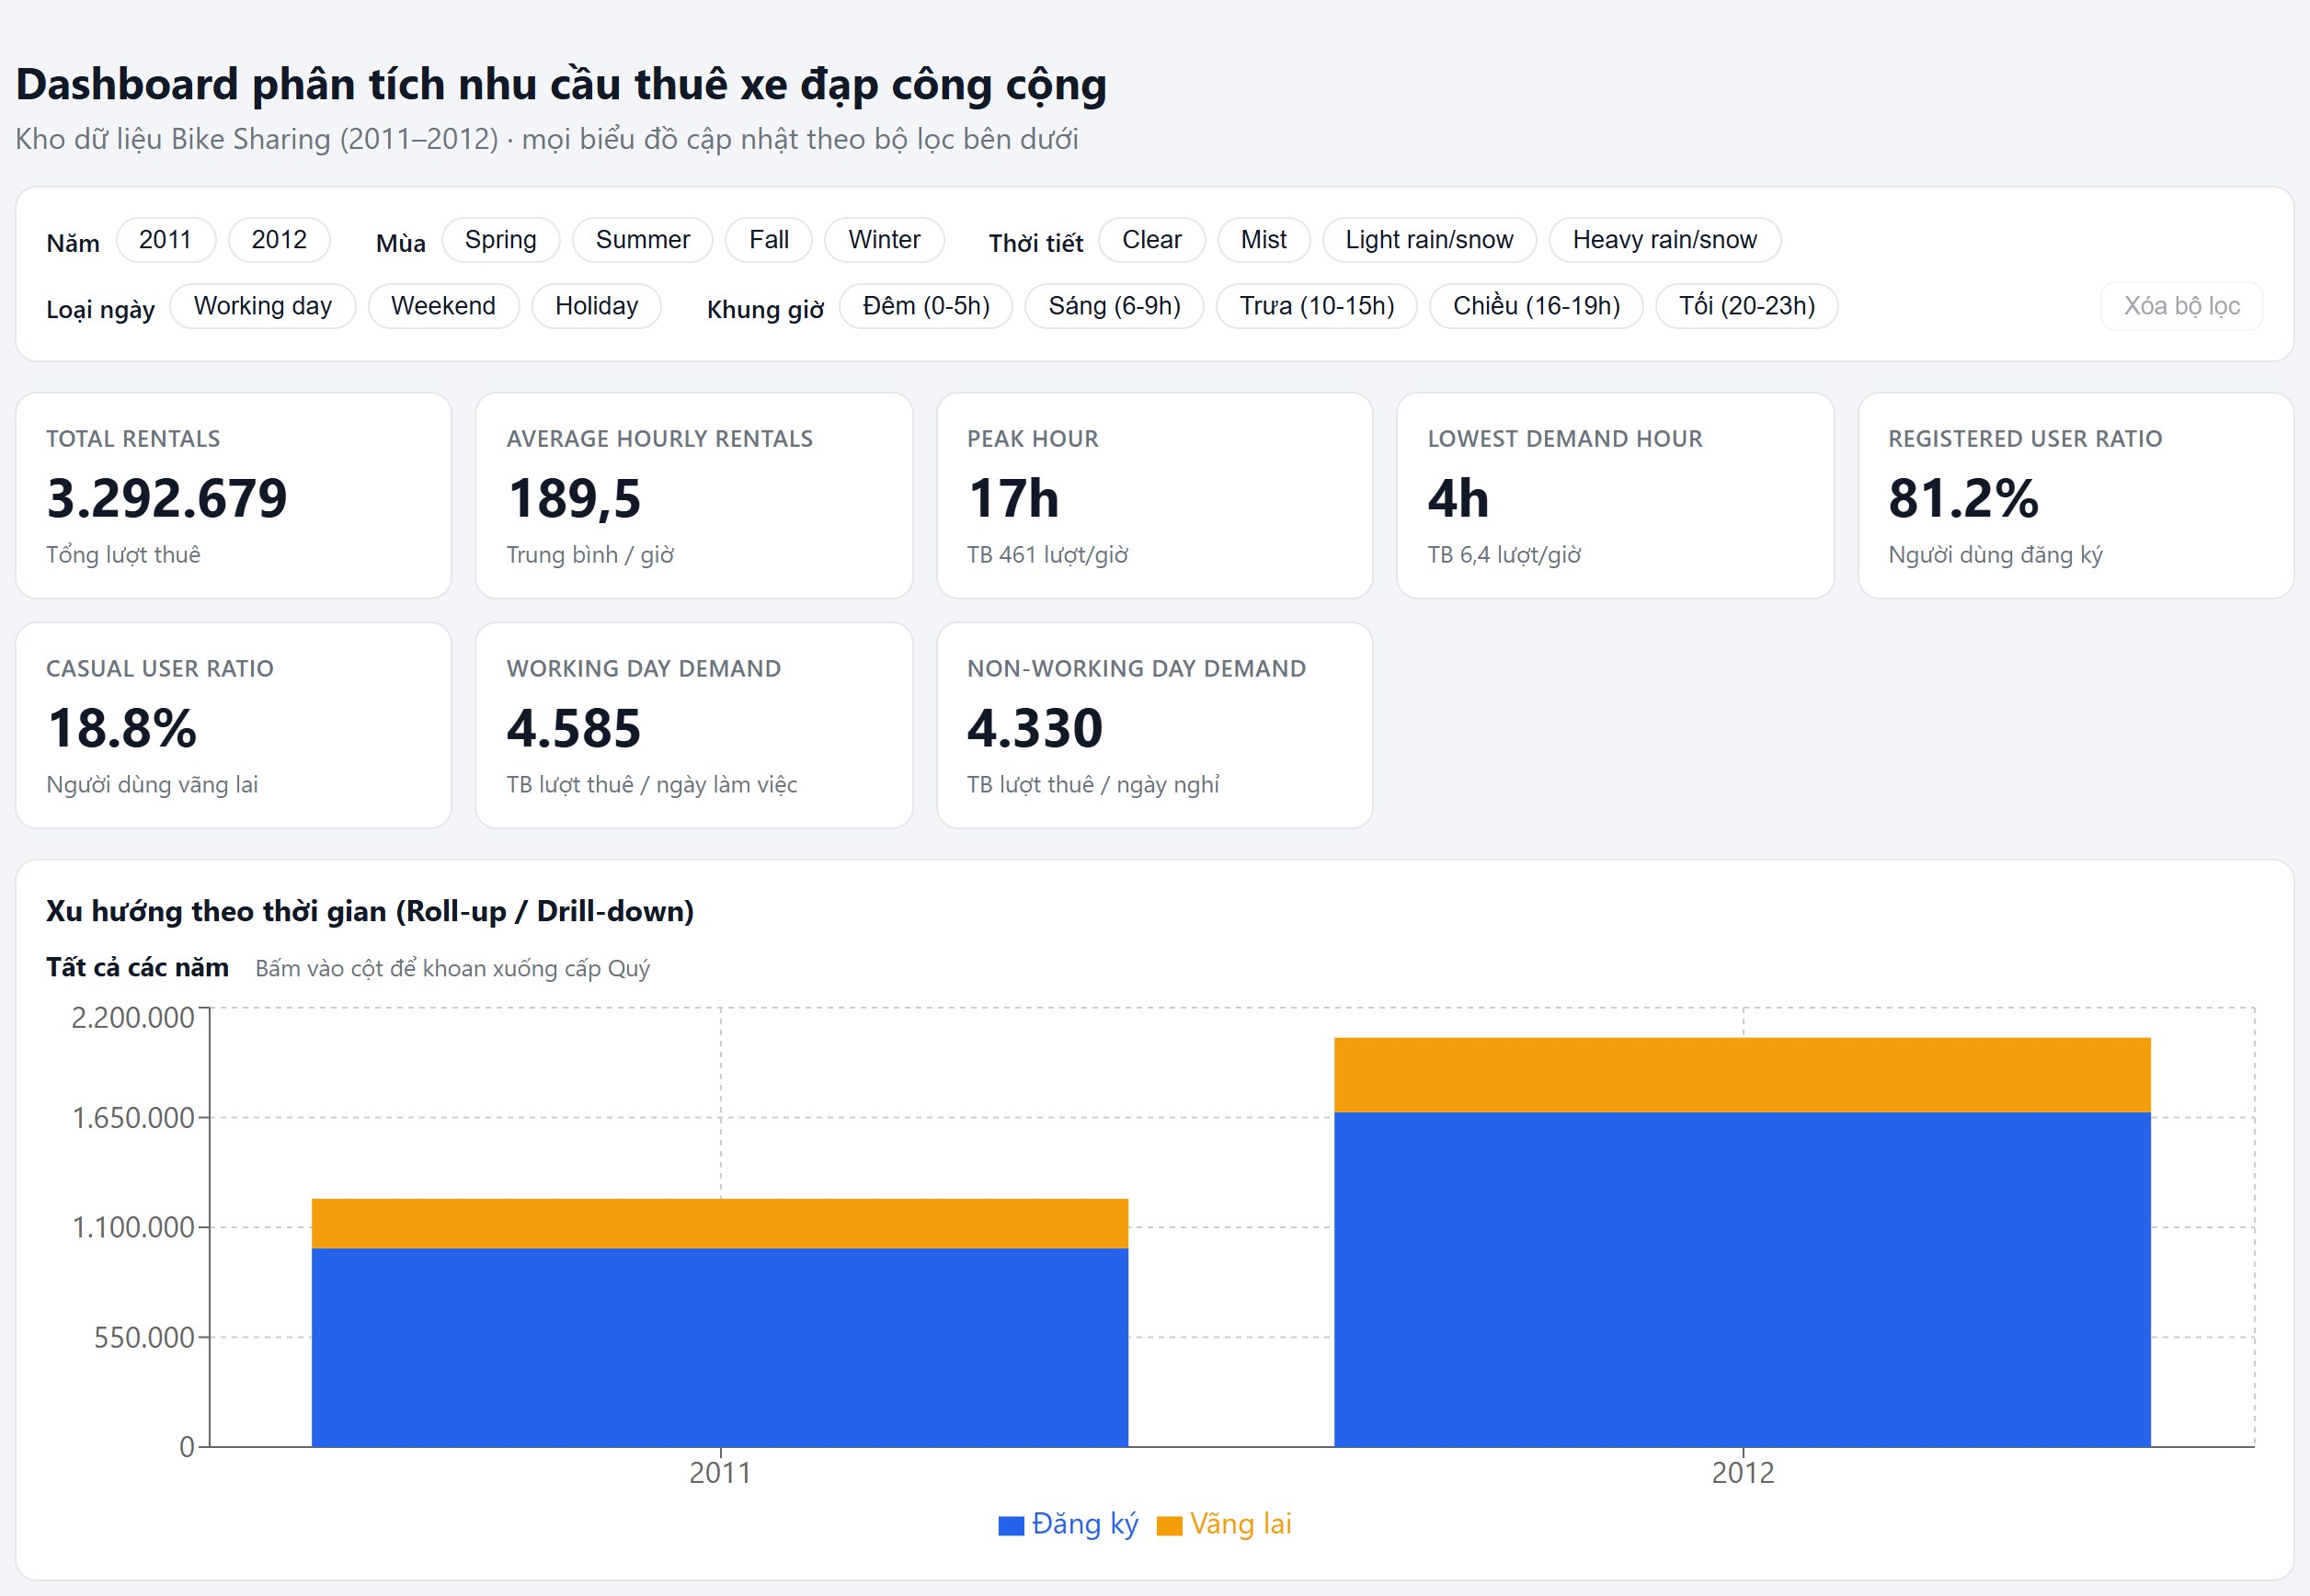
\includegraphics[width=\textwidth]{figures/dash_overview.jpg}
\caption{Dashboard: bộ lọc, 8 KPI và biểu đồ drill-down theo thời gian}
\label{fig:dash-overview}
\end{figure}

\begin{figure}[H]
\centering
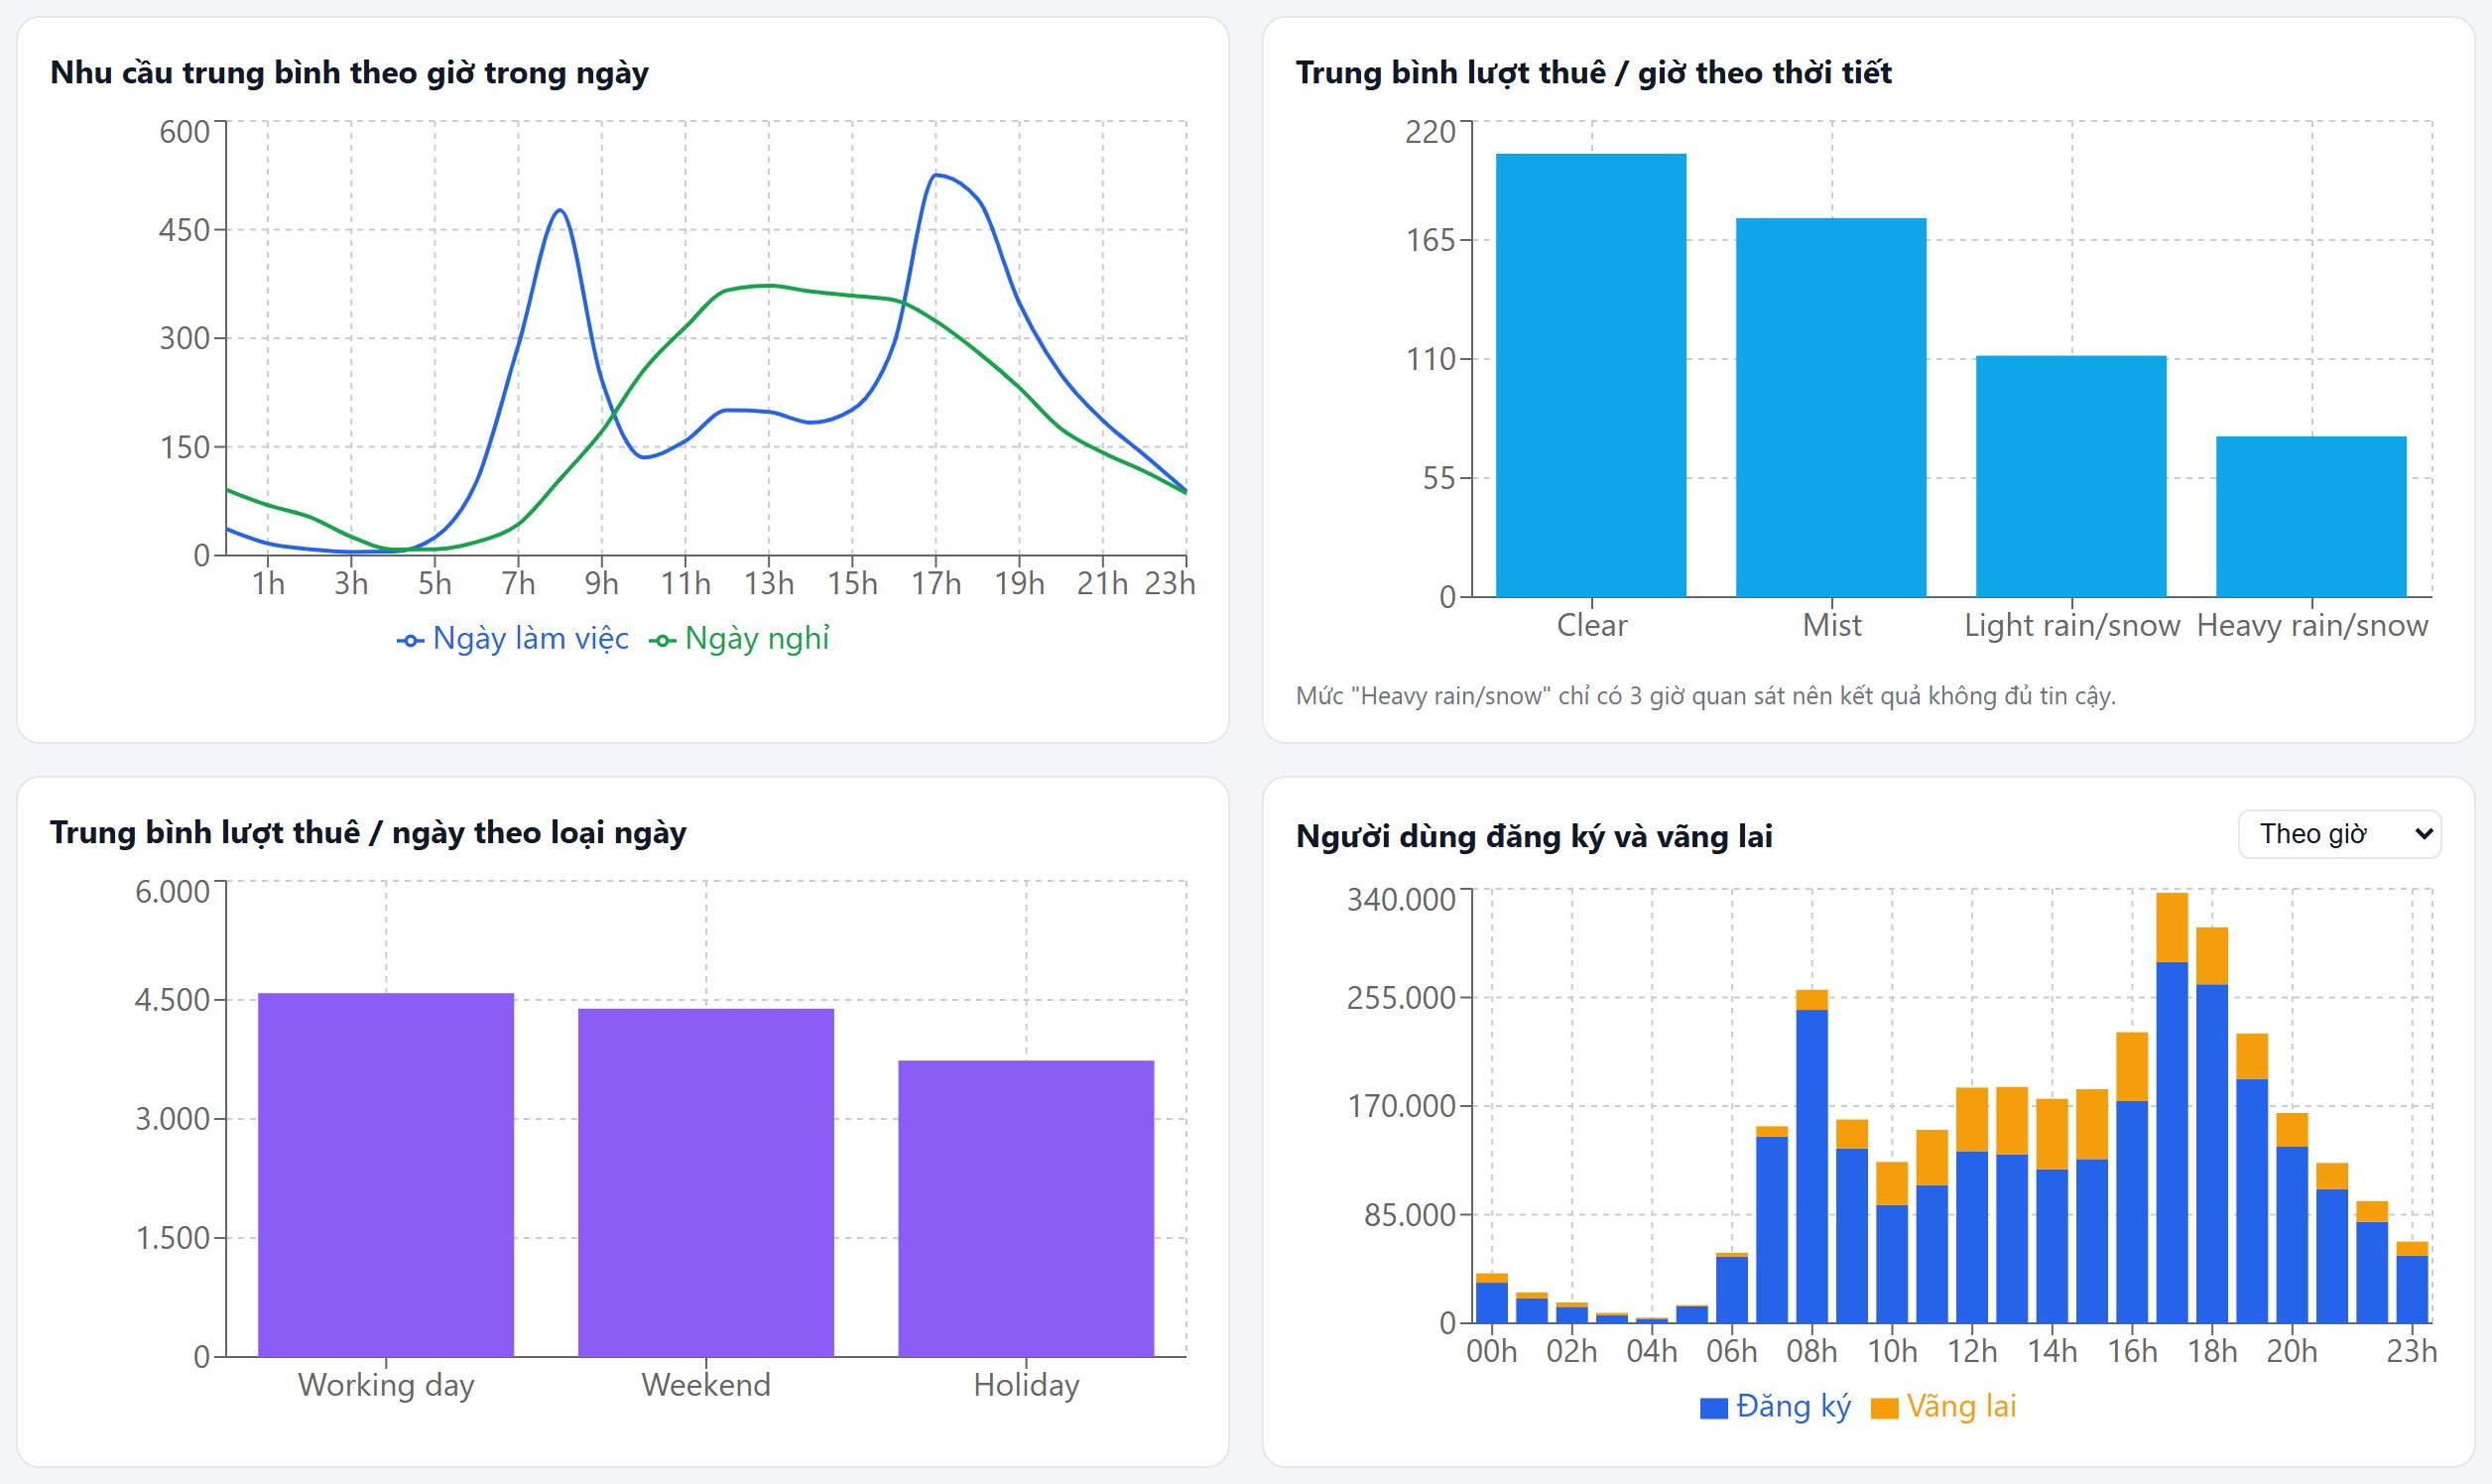
\includegraphics[width=\textwidth]{figures/dash_analysis.jpg}
\caption{Dashboard: phân tích theo giờ, thời tiết, loại ngày và nhóm người dùng}
\label{fig:dash-analysis}
\end{figure}

\begin{figure}[H]
\centering
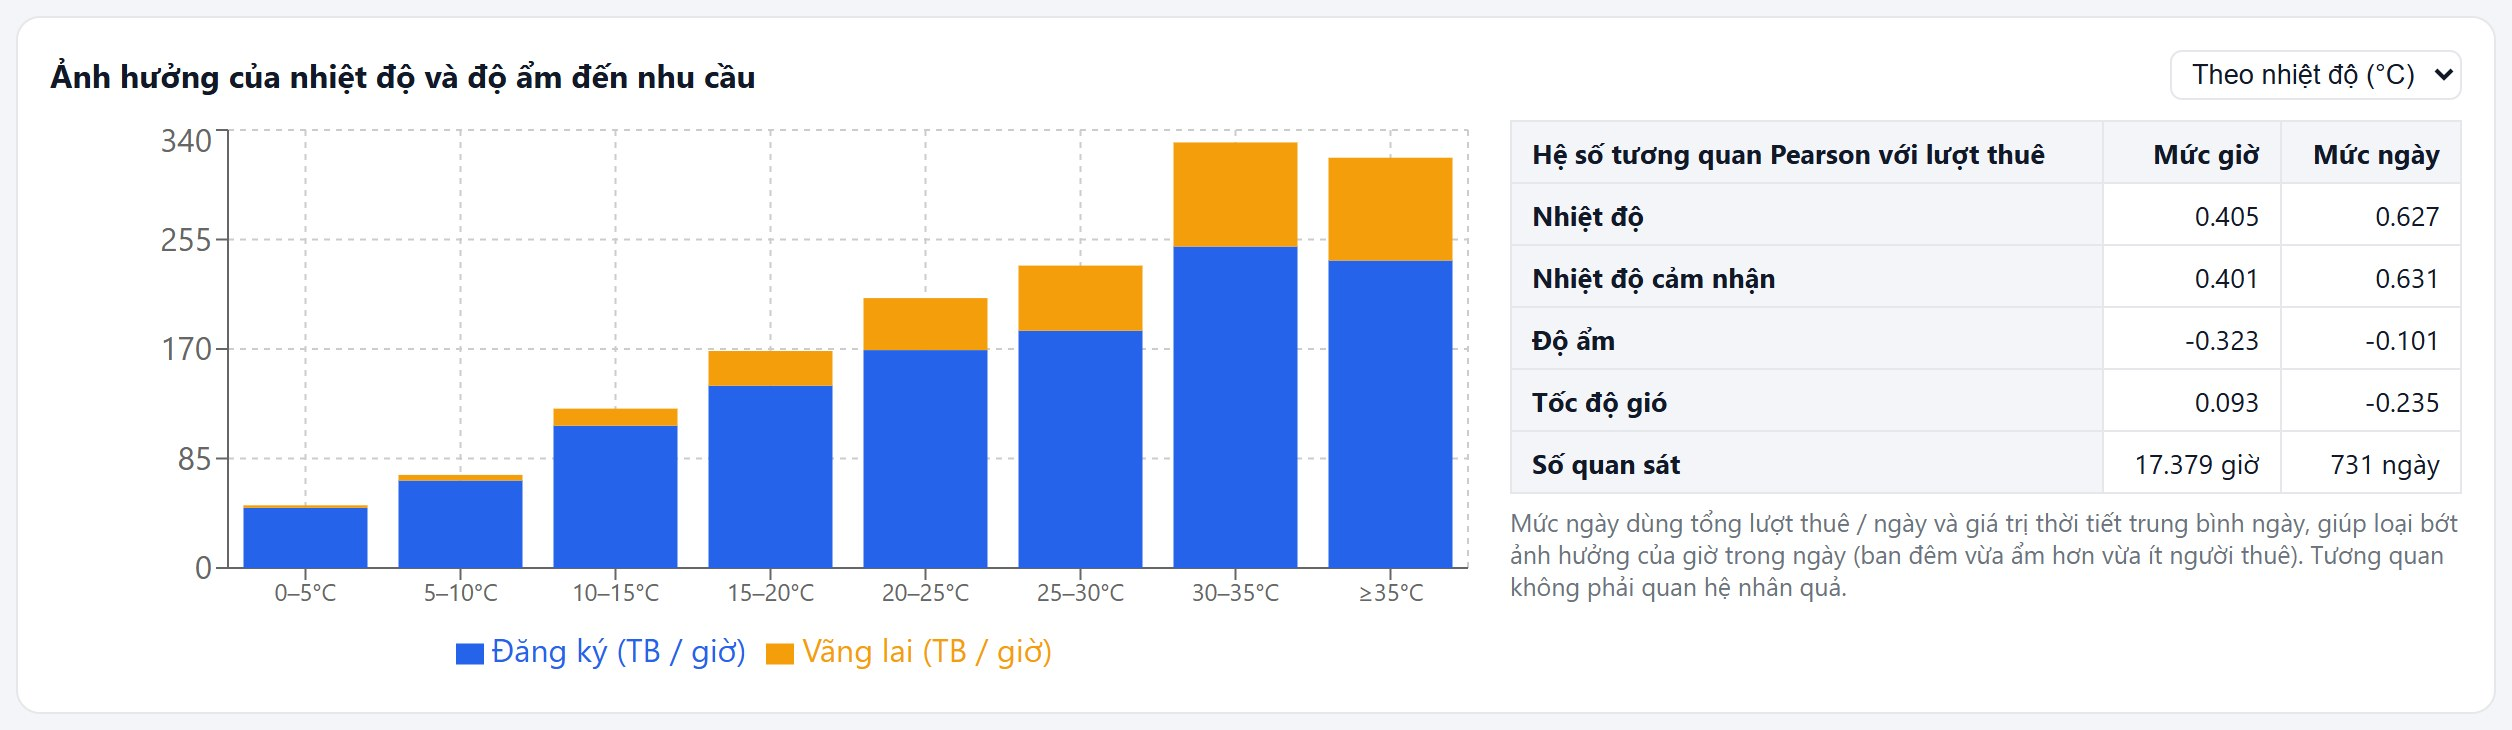
\includegraphics[width=\textwidth]{figures/dash_climate.jpg}
\caption{Dashboard: ảnh hưởng của nhiệt độ, độ ẩm và bảng hệ số tương quan}
\label{fig:dash-climate}
\end{figure}

\begin{figure}[H]
\centering
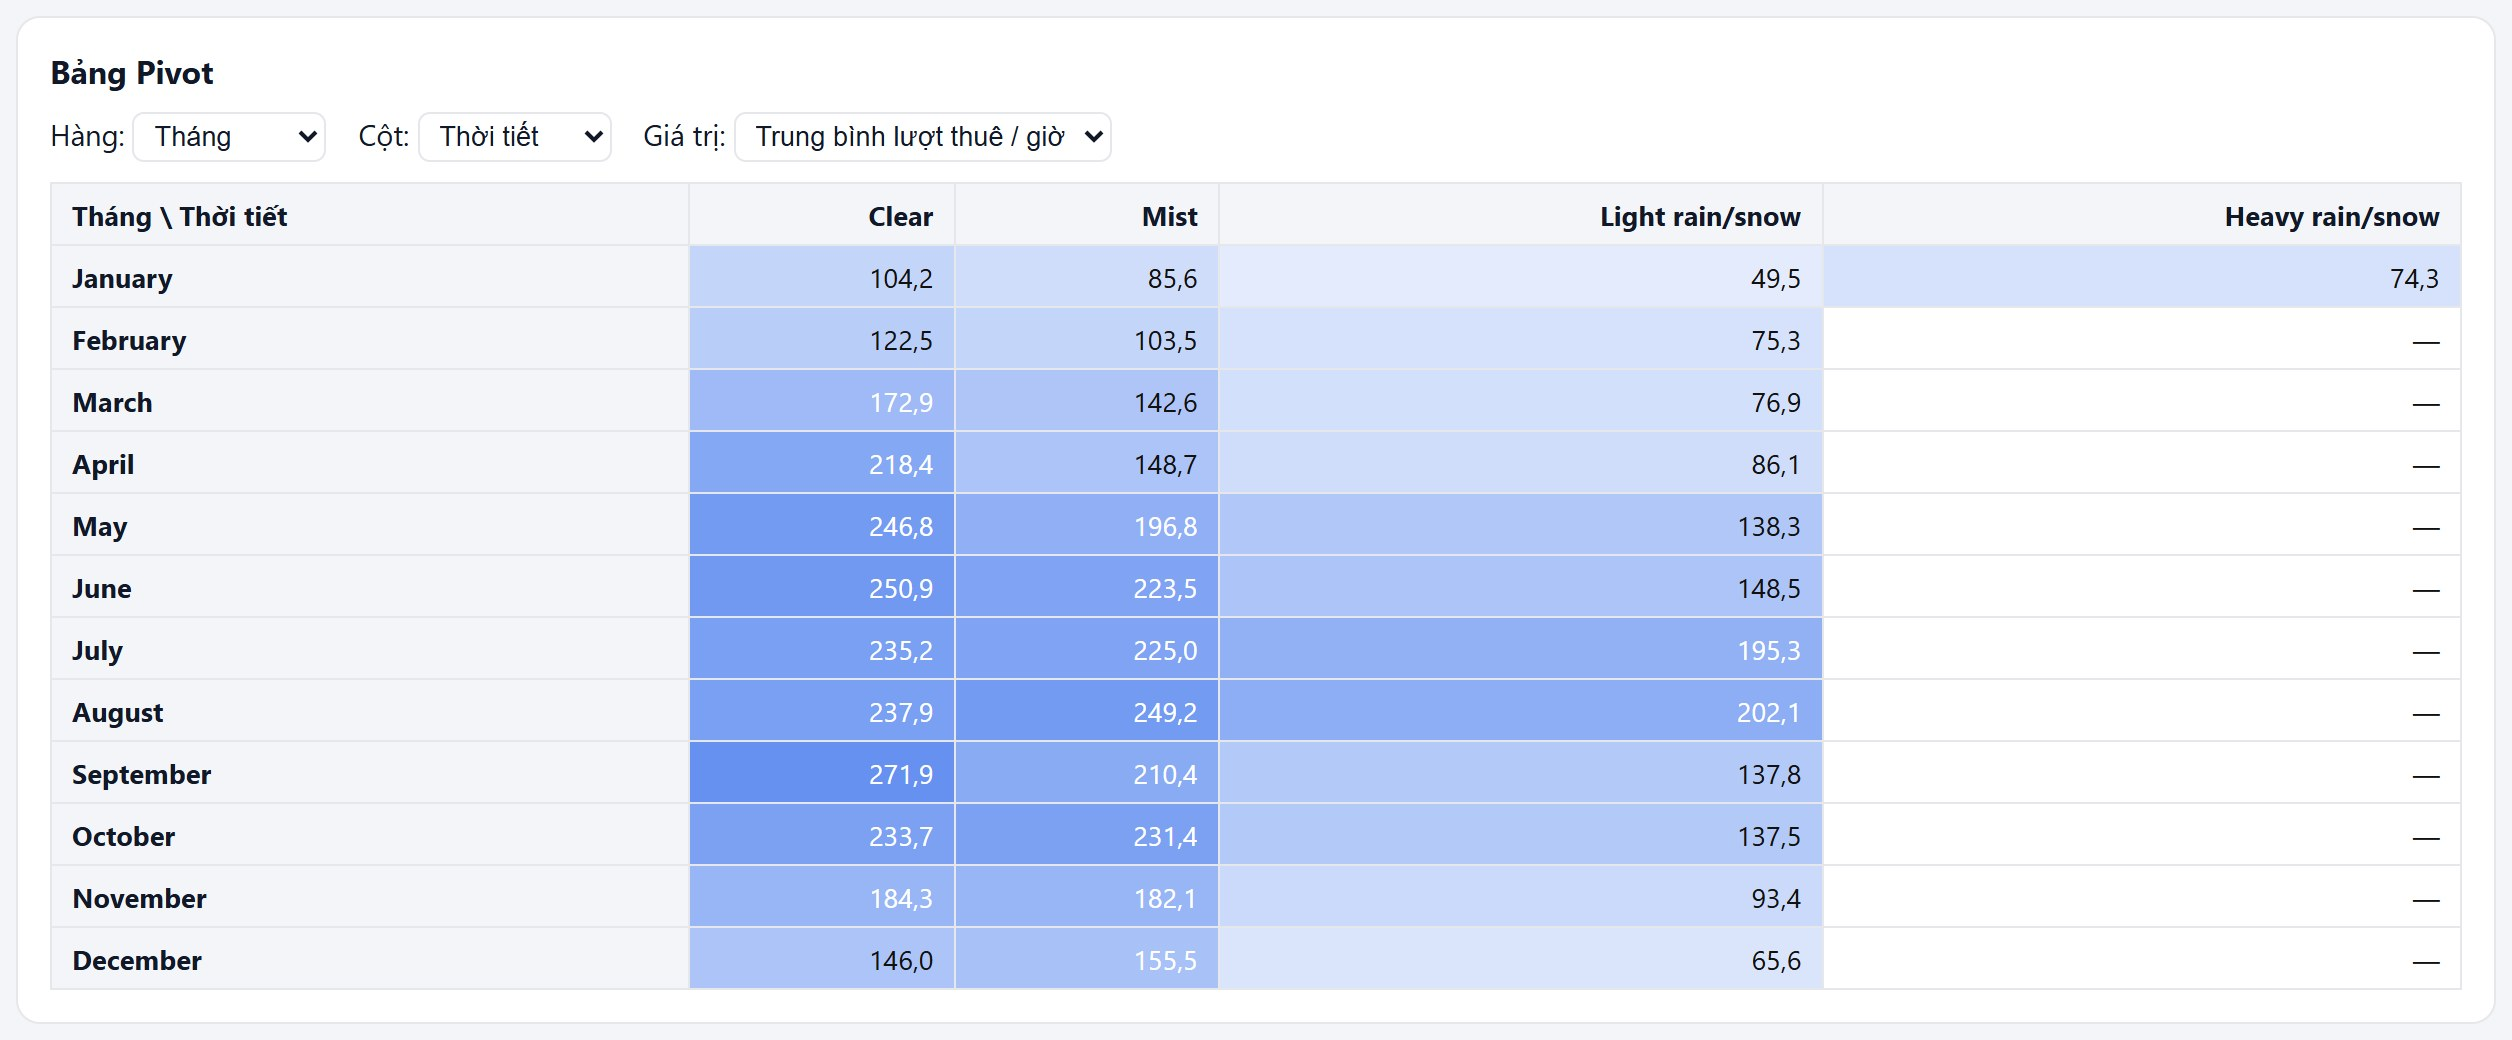
\includegraphics[width=\textwidth]{figures/dash_pivot.jpg}
\caption{Dashboard: bảng pivot tháng $\times$ thời tiết}
\label{fig:dash-pivot}
\end{figure}
